\chapter{Stopped flow \SOtwo measurements}\label{ch:stoppedflow}

As a first step in this research, experiments on blood using a stopped flow setup were completed, using a similar protocol and design used in previous work by the group.
These experiments used the stopped flow experimental setup from \autoref{ch:exptsetup}, with 3 different magnet systems at different fields to observe changes in \Ttwo at a number of levels of oxygenation.

\section{Experimental Protocol}
For this series of experiments, measurements of \Ttwo were made at a series of oxygenation steps, which we attempted to set by adjusting the gas mix going into the oxygenator.
These steps are shown graphically in TODO fig from ICMRM!!
After the flow circuit was assembled, the blood sample was loaded into the tubes and oxygenator, using the standard connectors on the bag.
The pump was switched on, and gas at 21\% \Otwo was flowed through to bring the oxygenation and temperature of the blood up to the 100\% starting point for the experiments.
The blood was allowed to flow through the circuit for TODO how long?? to stabilise, before an initial test with the iStat.
Durig this time, the probes were tuned and matched, and pulse sequence parameters such as pulse power were calibrated using amplitude sweeps (using FID on the Halbach system, and CPMG detection on the MOLE.)

If this showed that the pH, \SOtwo and HcT were normal, the flow was stopped and measurements on the two in-line NMR systems were started.
Typically \TR = \SI{1.5}{s}, with echo times of \SIlist{0.25;0.5;1;5}{ms} on the Halbach, and \SIlist{0.25; 0.5; 1}{ms} on the MOLE (these were limited by the magnetic field gradients in each system).
The number of echoes was adjusted to create an echo train \SI{600}{ms} long.
4 scans with phase cycling were used on the Halbach, but the poorer signal to noise on the MOLE meant that 16 scans were required.
Once these measurements had completed, the pump was turned on briefly to agitate the blood and minimize any effects of settling before repeating the NMR measurements.
A \SI{2}{ml} sample of blood in the circuit was also taken out and syringed into a clean \SI{5}{mm} NMR tube for the Spinsolve measurements.
These tubes were sealed with the caps provided by the manufacturer.
On the Spinsolve, typical experimental parameters were \TR = \SI{20}{s} with a 4 scan phase cycle, and with 4 echo times: \SIlist{0.5;2.5;5;10}{ms}.
Again, the number of echoes was set to give an echo train with a fixed length of \SI{10}{s}.

The \SOtwo was then lowered to an intermediate value (around 50\%).
Flow was turned back on and the gas mix set to 5\% \Otwo, which we had found produced these levels of oxygenation.
After waiting for the \SOtwo to reach the desired level, a sample of blood was taken from the flow circuit and the iStat was used to confirm the \SOtwo.
The flow was stopped, and two sets of NMR meaurements were completed as above, with samples also removed for the Spinsolve.

This process was repeated again to measure \Ttwo at a very low oxygenation (10\% or less), by setting the gas mix to 0\% \Otwo.
Afterwards, these steps were reversed to increase the oxygenation again, taking a measurement at an intermediate value of \SOtwo on the way up as well.

Data was extracted and processed using Python, in JuPyter notebooks.
Each echo train is phased, and each echo is summed to give a single value for the signal at each echo time.
The resulting decay is fit to a monoexponential decay using non-linear least squares fitting, which results in a single \Ttwo value at each \SOtwo.

\section{Results}
\subsection{Spinsolve results}
Two examples of the CPMG decays measured on the Spinsolve are shown in \autoref{fig:sf-spinsolveCPMG}.
Plotting the log of the echo amplitudes against time gives a straight line, which indicates that the decay is mono-exponential.
This agrees with what is reported in the literature.

This data also shows even-echo rephasing occuring in the decays measured with long echo times (in red).
Where this was visible, only the even echoes were used in the curve fitting routine to find \Ttwo.

%Graph generated in processBloodOxygenation1/Spinsolve data 170728
\begin{figure}[bh]
\centering
\begin{subfigure}[t]{0.48\textwidth}
\caption{\SOtwo = 95\%}
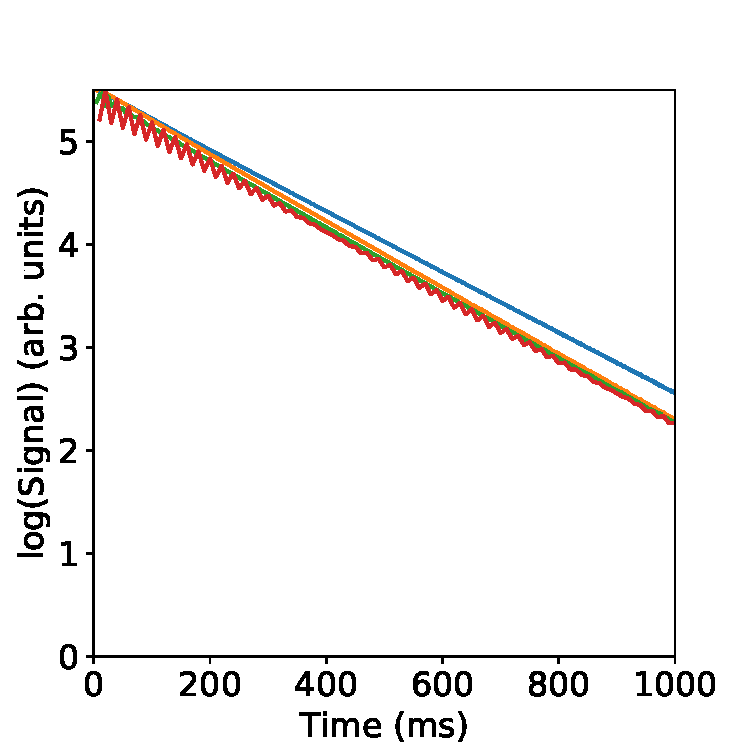
\includegraphics[width=\textwidth]{figures/stoppedflow/spinsolveCPMG95.pdf}
\end{subfigure}
\begin{subfigure}[t]{0.48\textwidth}
\caption{\SOtwo = 9\%}
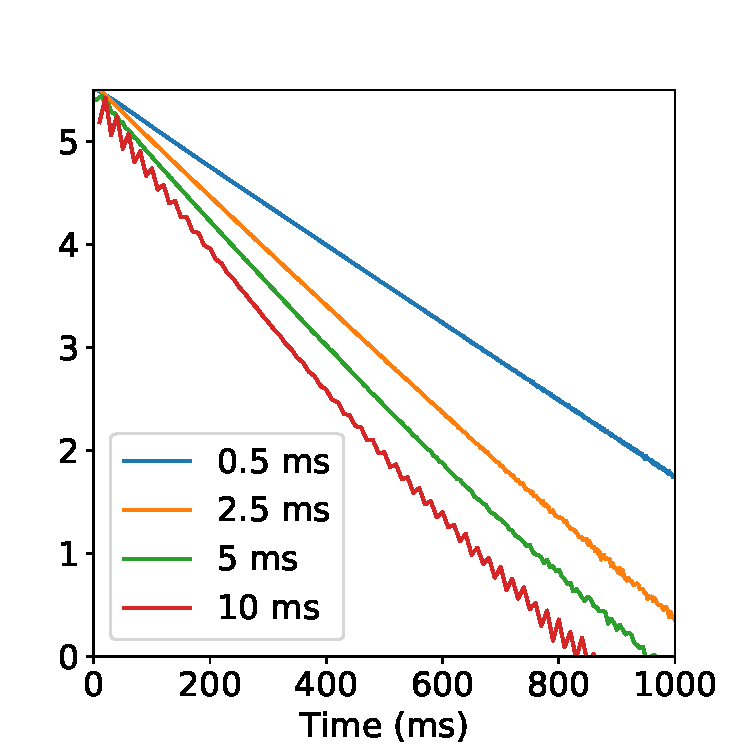
\includegraphics[width=\textwidth]{figures/stoppedflow/spinsolveCPMG9.pdf}
\end{subfigure}
\caption{Examples of CPMG decays measured on the Spinsolve for oxygenated and deoxygenated blood}
\label{fig:sf-spinsolveCPMG}
\end{figure}

Decays were measured at a range of oxygenations and fitted to obtain \Ttwo.
These results are shown in \autoref{fig:sf-spinsolveT2SO2}.

%Graph generated in processBloodOxygenation1/Spinsolve data 170728
\begin{figure}[ht]
\centering
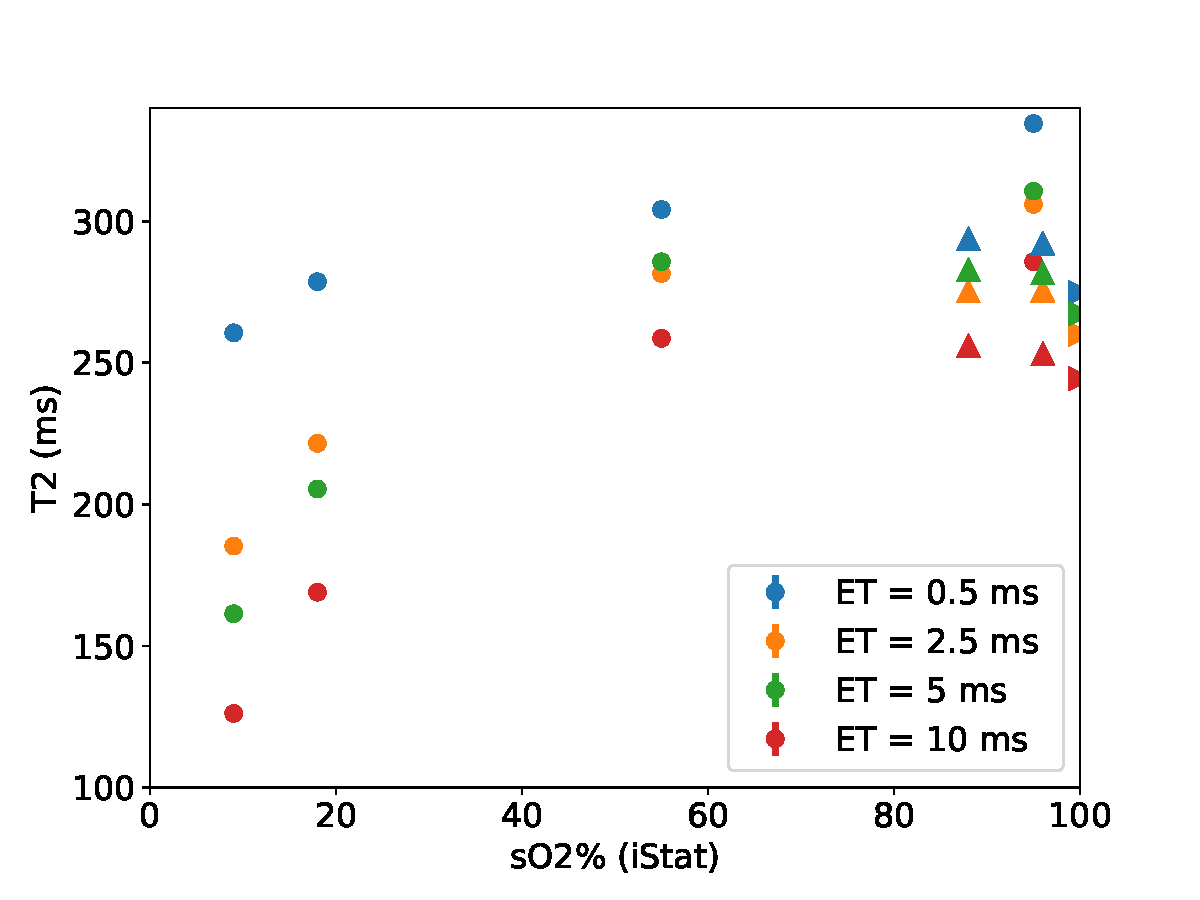
\includegraphics[width=\textwidth]{figures/stoppedflow/spinsolveT2SO2down.pdf}
\caption[\Ttwo vs. \SOtwo measured on the Spinsolve]{\Ttwo at different levels of oxygenation, measured on the Spinsolve. Circles indicate samples measured when deoxygenating the blood, while upwards pointing triangles are samples when oxygenating it (see experimental protocol). Right pointing triangles are a sample hyperoxygenated with 30\% \Otwo}
\label{fig:sf-spinsolveT2SO2}
\end{figure}


As the oxygenation of the blood was lowered, the \Ttwo decreases from \SI{334}{ms} to \SI{260}{ms} at the short echo time, while changes more drastically from \SI{285}{ms} to \SI{126}{ms} at the longest echo time.
This shows that the changes in oxygenation are visible in this \SI{1}{T} system.
The shorter \Ttwo at long echo time is expected, as there is more time for dephasing to occur, as discussed in TODO backgroundsection!!.
The separation between the short echo time and long echo time \Ttwo{}s also increases at lower \SOtwo.
This is predicted by theory, as the susceptibility difference and induced field inhomogeneity is increased with high levels of deoxyhaemoglobin.

One difficulty we had was recovering the original \Ttwo value when the blood was re-oxygenated.
This is shown by the two samples measured while oxygenating (triangles in \autoref{fig:sf-spinsolveT2SO2}.
A number of experiments were conducted to investigate the cause of this, and these are discussed below TODO discussions!!.


\subsection{Halbach results}
%Graph produced in Halbach 170726


The Halbach magnet system was run inline with the flow circuit, making it easier to measure more data points.
As with the Spinsolve results, the CPMG decays were found to be monoexponential, however there was no appearance of even echo rephasing in the CPMG decays.
In this experiment, the deoxygenation causes the \Ttwo to decrease from \SI{337}{ms} to \SI{303}{ms} fot the short echo time, and from \SI{226}{ms} to \SI{152}{ms} for the \SI{5}{ms} echo time.
The strong field gradients in this system means that the CPMG experiments are sensitive to the diffusion of protons moving through the gradient, which causes longer echo times to measure a shorter \Ttwo.
This can be seen in the position of the \SI{5}{ms} points (red), which are significantly lower than points at \textless\SI{1}{ms}.
In this experiment, measurements were also completed with echo times of \SIlist{8;12}{ms}, but these did not show any trends due to the strong relaxation from the field inhomogeneities.

\begin{figure}[ht]
\centering
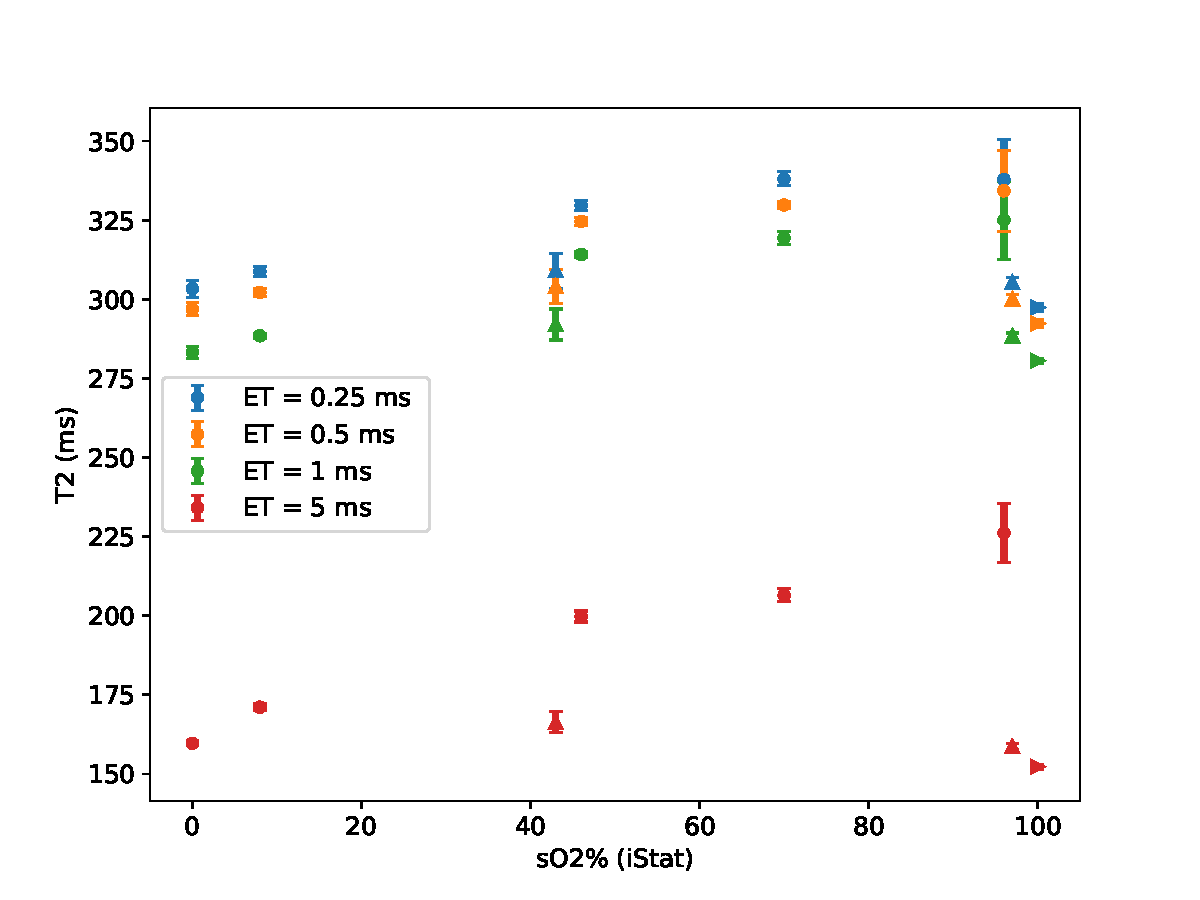
\includegraphics[width=\textwidth]{figures/stoppedflow/halbachT2SO2.pdf}
\caption[Stopped flow \Ttwo vs. \SOtwo measured on the Halbach system]{\Ttwo vs. \SOtwo measured on the Halbach system. Circles indicate samples measured when deoxygenating, upwards triangles are measured when oxygenating and right-pointing triangles are a sample oxygenated with 30\% \Otwo. Error bars represent standard error (n=3)}
\label{fig:sf-halbachT2SO2}
\end{figure}

Like the Spinsolve experiments, the \Ttwo values in this experiment did not reach the same levels they did at the start of the experiment, which suggests that the state of the blood in the circuit has changed.

\subsection{MOLE results}
%Graph from Mole 170728
Measurements on the MOLE had much less signal to noise than the other two systems.
This is related to both the reduced field strength \SI{0.1}{T}, and the single-sided design of the magnet system.
Because of this, measurements took longer to acquire than on the other systems and the largest source of experimental uncertainty was from the fitting process.


\section{Discussions}

\begin{itemize}
\item Hard to set sO2 with gas mixer
\item decreasing \Ttwo when hyperoxygenating?, connection to literature
\item Effect of blood settling when flow stopped
\item time taken to measure sO2 with iStat
\end{itemize}
